\chapter{Wstęp}
\section{Cel}
Celem pracy inżynierskiej jest budowa środowiska symulacyjnego robota mobilnego z kołami szwedzkimi.
Dla realizacji tego celu należy opracować model 3D, oraz model dynamiki dookólnej bazy jezdnej z 4 kołami szwedzkimi.
Jednym z przyjętych założeń jest wymaganie, aby opracowany model był możliwie dokładny i jego działanie było zbliżone do rzeczywistego robota.
Opisywana platforma będzie używana jako baza wielokierunkowa do przemieszczania dwuramiennego robota manipulacyjnego Velma.

Celem jest stworzenie modelu, który będzie reagował na siły podobnie do rzeczywistego robota i był sterowany tak samo, jak rzeczywisty robot.
To spowoduje, że możliwe będzie stworzenie jednego wspólnego programu sterującego do użycia zarówno w symulacji, jak i rzeczywistym robocie.

Testowanie oprogramowania sterującego na rzeczywistym obiekcie może prowadzić do jego uszkodzeń, dlatego wpierw należy się upewnić o poprawności projektowanych rozwiązań na bezpiecznym modelu wirtualnym.
Rzeczywistość nie pozwala także na skomplikowane scenariusze testów, które w rzeczywistości mogłyby być niemożliwe do wykonania lub koszty jego wykonania byłyby zbyt wysokie.
Szybciej i taniej jest stworzyć symulacyjne środowisko testowe, niż fizyczne, w dodatku błąd sterowników przy symulacji nie grozi zniszczeniem rzeczywistego robota.
Dopiero przy osiągnięciu satysfakcjonującej jakości sterowania w symulacji wirtualnej można zastosować algorytmy sterowania do rzeczywistego obiektu bez ryzyka uszkodzeń urządzenia.

Oprócz modelu bazy jezdnej, środowisko symulacyjne musi również udostępniać modele czujników, w które wyposażony jest robot. 
Odczyty z symulatorów czujników są następnie wykorzystywane w układzie sterowania do generacji odpowiednich sygnałów sterujących.
W celu możliwie wiernej symulacji działania czujników do wartości pomiarów dodaje się szum pomiarowy i zakłócenia.


\section{Dookólna platforma mobilna}
\begin{figure}[H]
\centering
 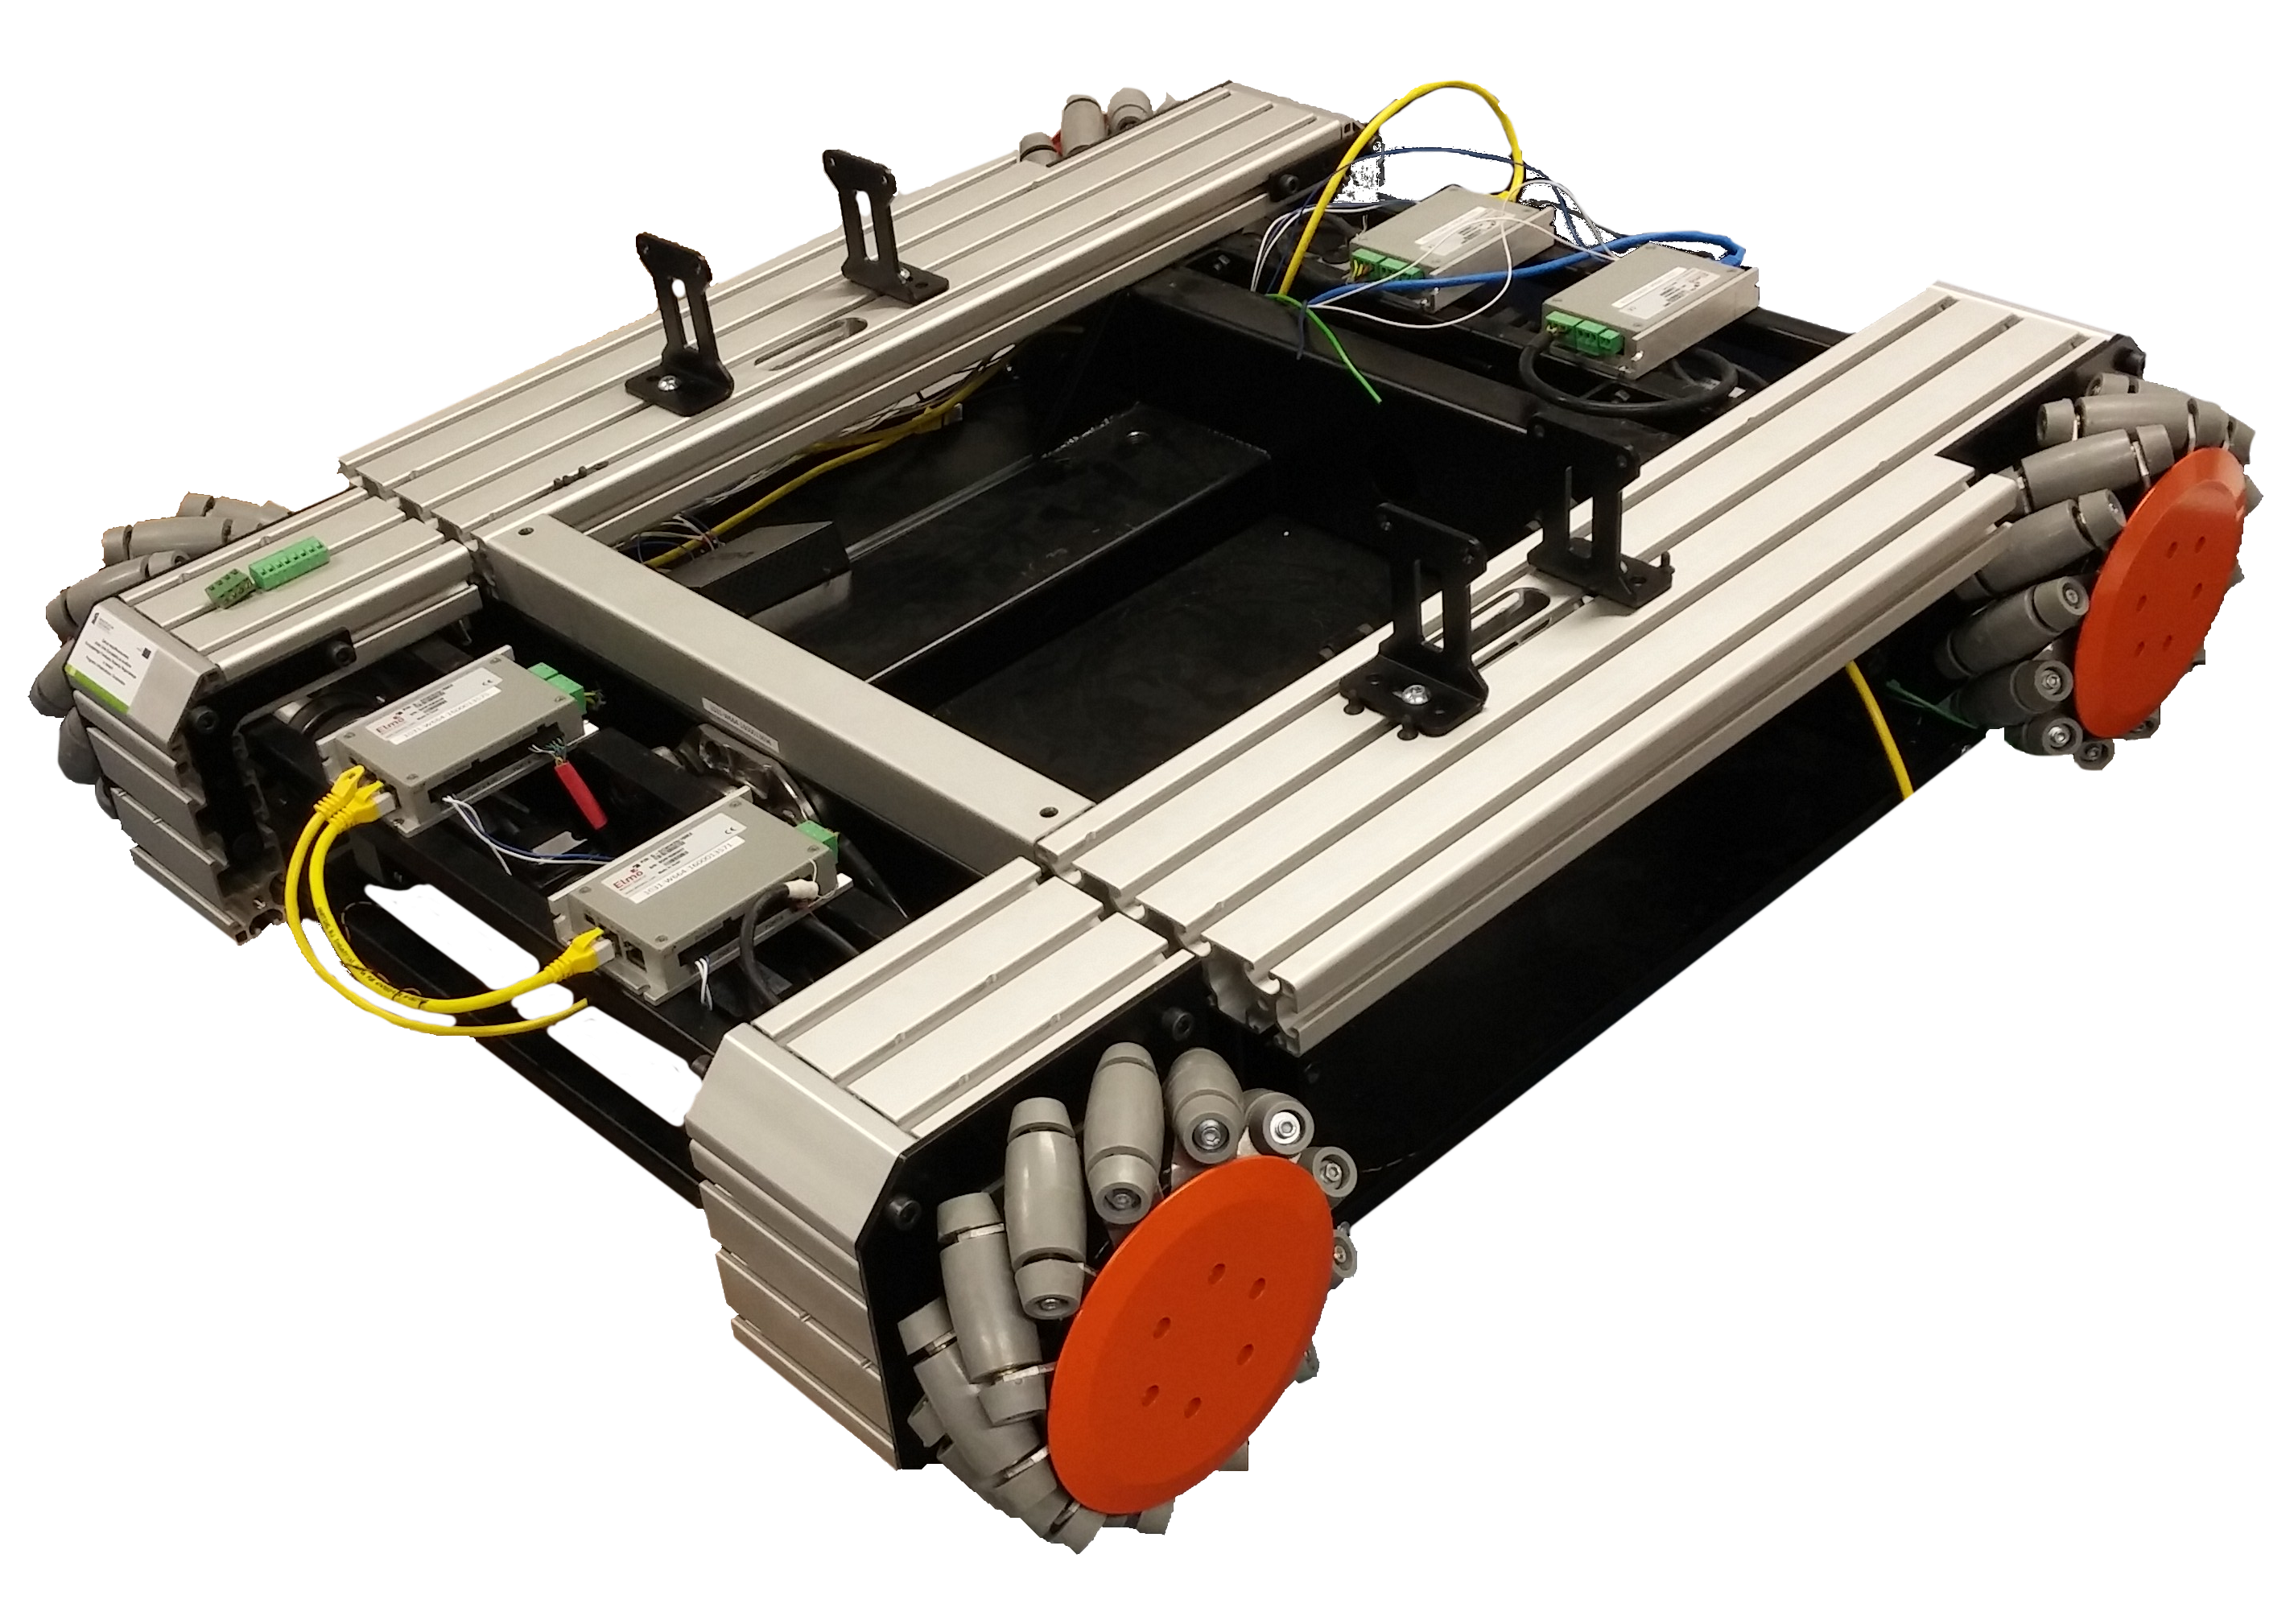
\includegraphics[width=0.8\textwidth]{graphics/base_photo.png}
\caption{Dookólna baza mobilna na kołach szwedzkich.}
\label{fig:base_photo}
\end{figure} 

Jest to duża, prostokątna baza dookólna poruszająca się na czterech kołach szwedzkich, patrz fotografia \ref{fig:base_photo}.
Koła są stałe, parami przytwierdzone do dwóch osi.
Każde koło jest sterowane osobno przez podłączony bezpośrednio serwomotor, zatem może mieć prędkość i kierunek niezależny od pozostałych kół, kierunku poruszania się robota, oraz jego obrotu.
Każdy z serwomotorów ma także wbudowany enkoder.
Sterownik enkodera zwraca aktualny kąt i prędkość obrotu.

Jest to najpopularniejsza budowa dookólnych platform mobilnych, mająca zastosowanie także w innych robotach, jak na przykład Kuka Youbot \ref{fig:kuka_youbot}.
Pomimo, że robot o trzech kołach szwedzkich i prostszej budowie ma taką samą ilość stopni swobody, to jego stabilność jest gorsza od czterokołowych wersji \cite{extra_axis}.
Ponieważ jest to robot transportowy, to stabilność odgrywa tu ważną rolę i czterokołowa budowa jest wskazana.

\begin{figure}[H]
\centering
 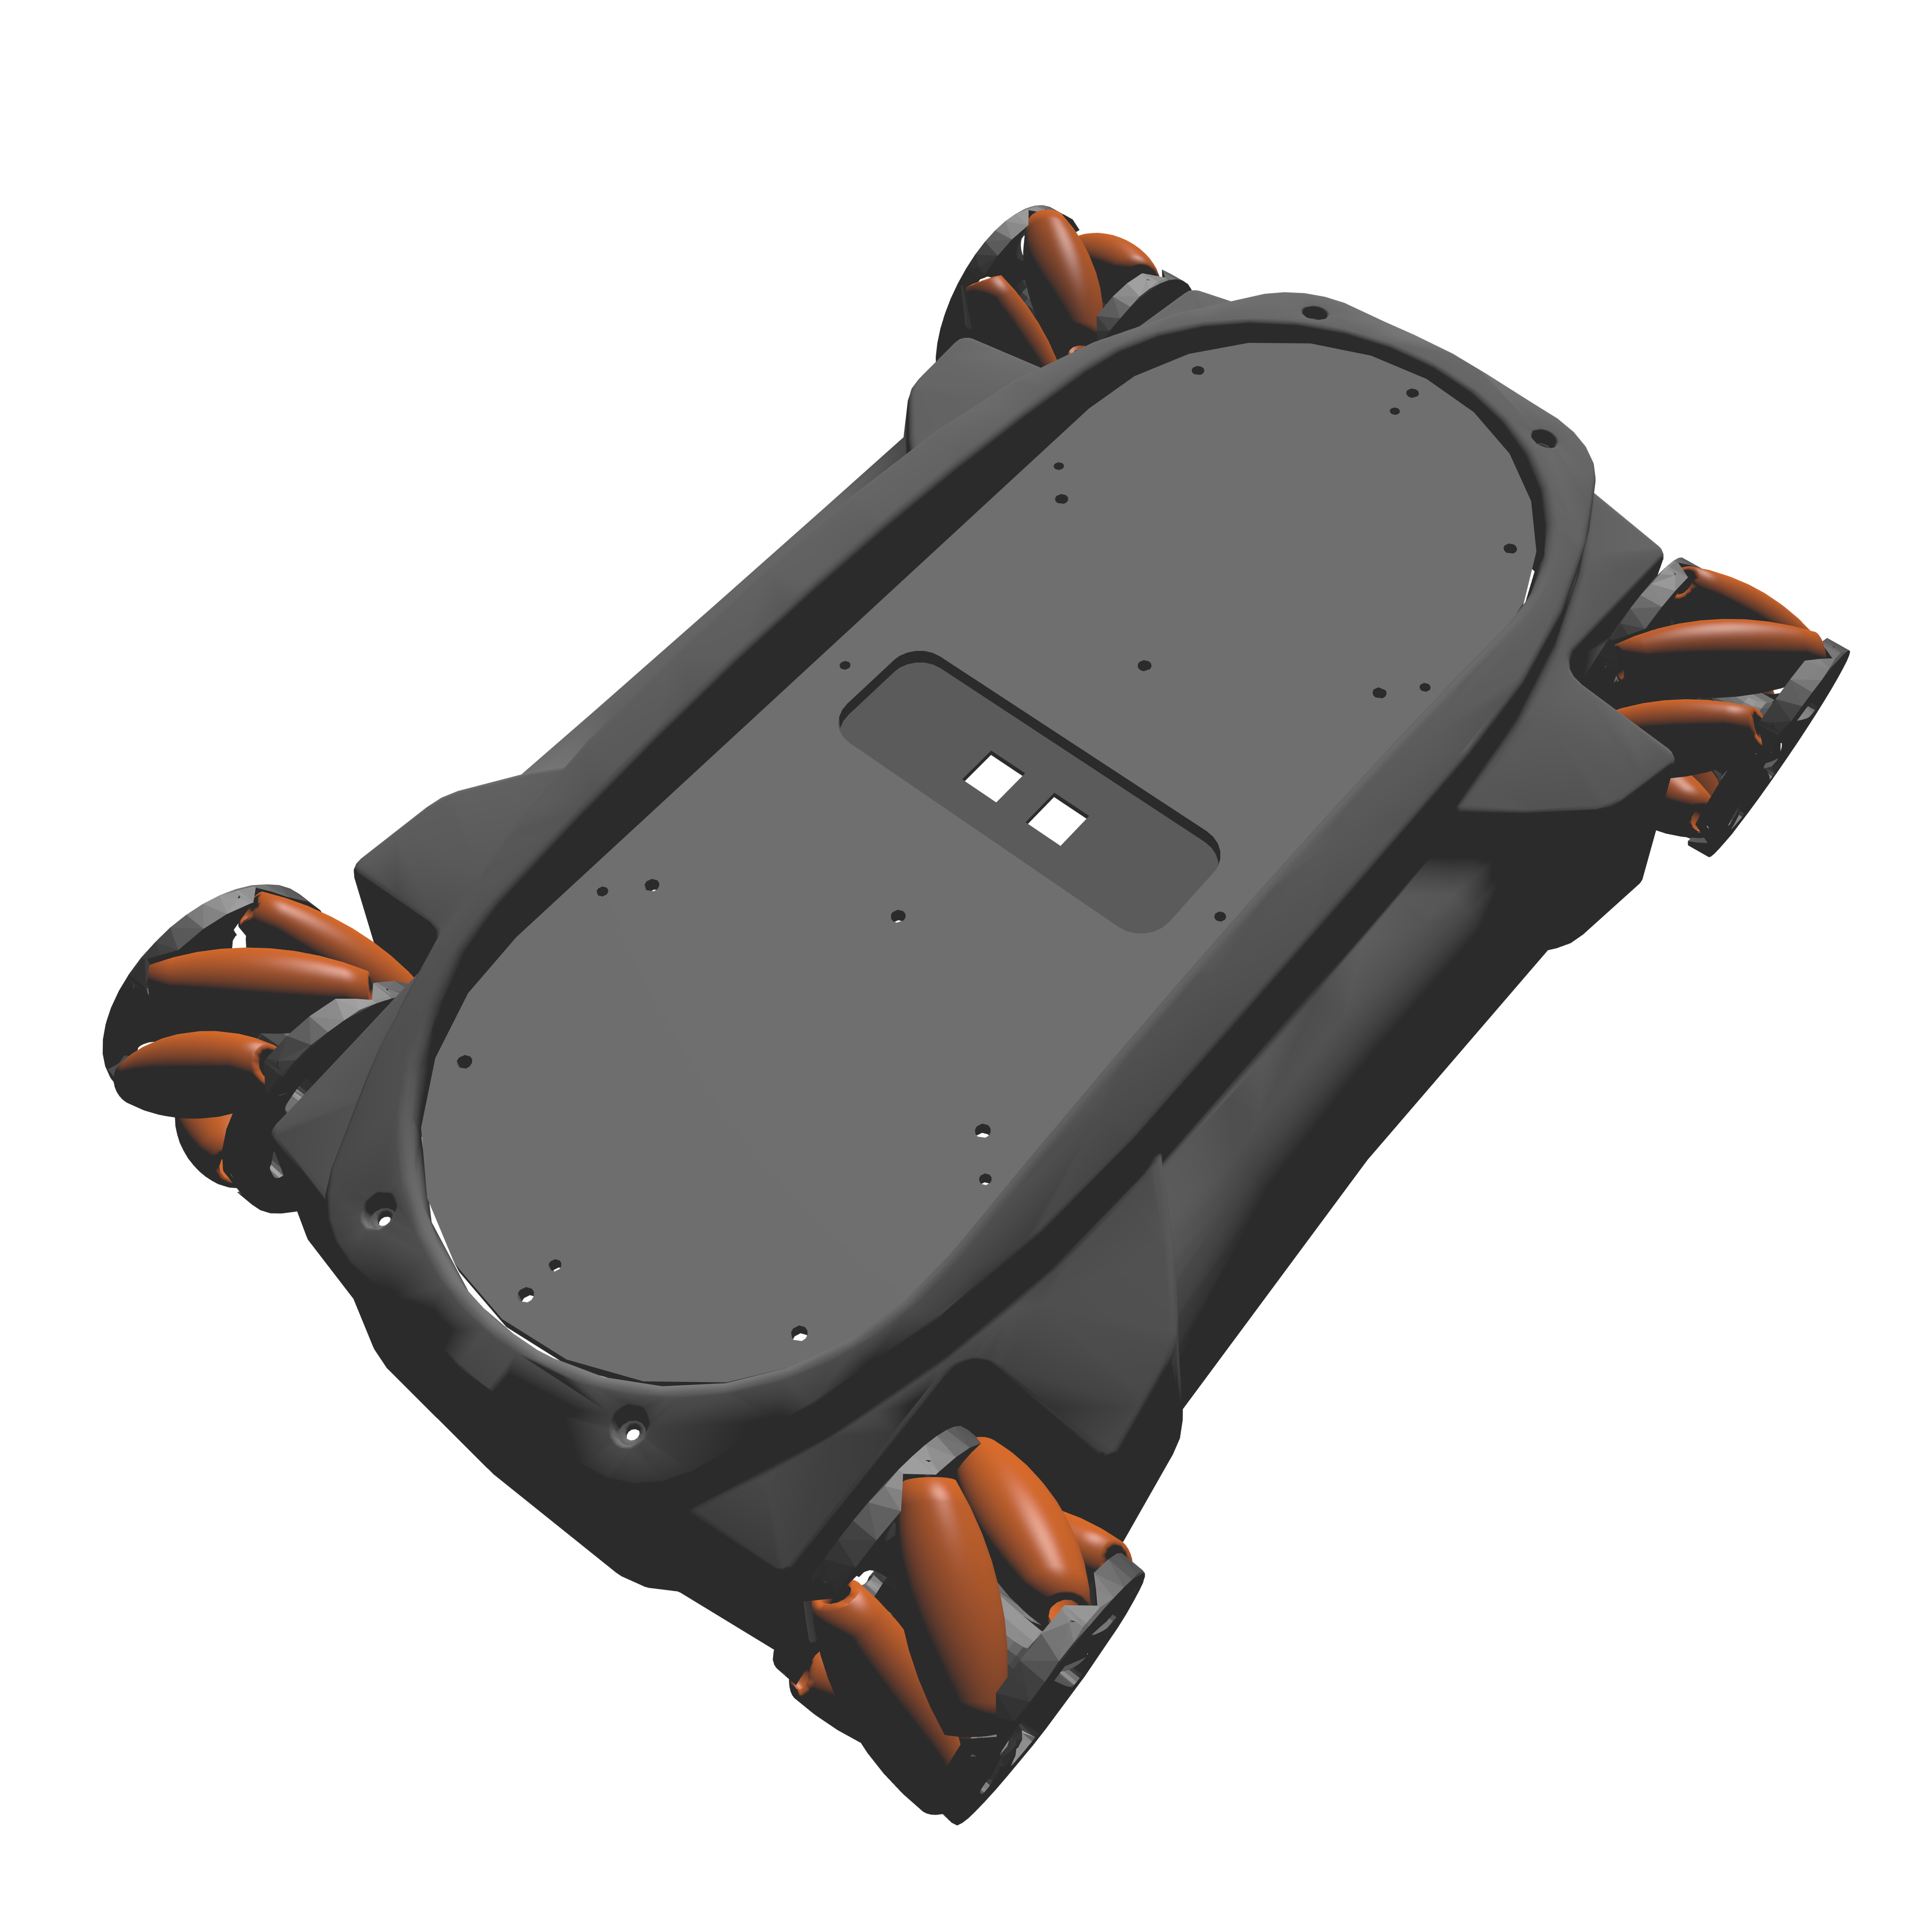
\includegraphics[width=0.5\textwidth]{graphics/kuka_youbot.png}
\caption{Przykład innej platformy wielokierunkowej na podstawie fragmentu komercyjnego robota Kuka Youbot. Należy zwrócić uwagę na charakterystyczne ustawienie kół, identyczne jak w opisywanej platformie \ref{fig:base_photo}.}
\label{fig:kuka_youbot}
\end{figure} 

Odpowiedni obrót kół względem bazy pozwala na jej ruch w dowolnym kierunku niezależnie od kąta obrotu robota, patrz rysunek \ref{fig:mecanum_dirs}.
Za ich pomocą da się także obracać bazą stojąc w miejscu, lub w trakcie ruchu po prostej.
Na przykład, jeśli obracać tylko przeciwległymi kołami po przekątnej, system zacznie się poruszać po skosie bez zmiany kąta obrotu.
A jeśli do tego dodamy obrót kół drugiej przekątnej w odwrotnym kierunku, wtedy pojazd zacznie się poruszać w bok pomimo faktu, że koła nie są skrętne i nie mogą ustawić się prosto do kierunku jazdy.
Trasa po której porusza się obiekt przy stałej prędkości kół zawsze jest okręgiem, możemy uznać prostą za okrąg o nieskończonym promieniu, a punkt za okręg o zerowym.
Wynika to z tego, że każdy obiekt, który ma jednostajną prędkość o kierunku w lokalnym układzie współrzędnych, oraz prędkość kątową będzie się poruszał po takiej krzywej.

\begin{figure}[H]
\centering
 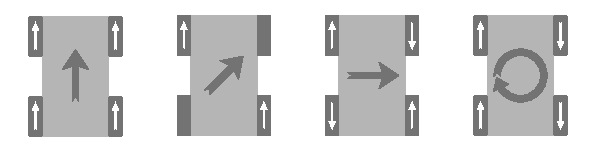
\includegraphics[width=0.8\textwidth]{graphics/mecanum_dirs.pdf}
\caption{Podstawowe ruchy, jakie może wykonywać robot o napędzie wielokierunkowym.}
\label{fig:mecanum_dirs}
\end{figure} 

Podstawa ma za zadanie transportować robota manipulującego Velma tworząc razem manipulator mobilny.
Velma to wysoki i bardzo ciężki robot wyposażony w dwa chwytaki na ramionach o wielu przegubach, patrz fotografia \ref{fig:velma}.
Taka budowa wymaga szerokiej podstawy, aby zachować dużą równowagę.
Jeżdżąc na tej podstawie robot może się przemieszczać i obracać w dowolnym kierunku, aby uzyskać lepszy dostęp do manipulowanych przedmiotów.
Dodatkowe czujniki laserowe umieszczone tuż nad postawą odpowiadają za wykrywanie kolizji i lokalizację.

\begin{figure}[H]
\centering
 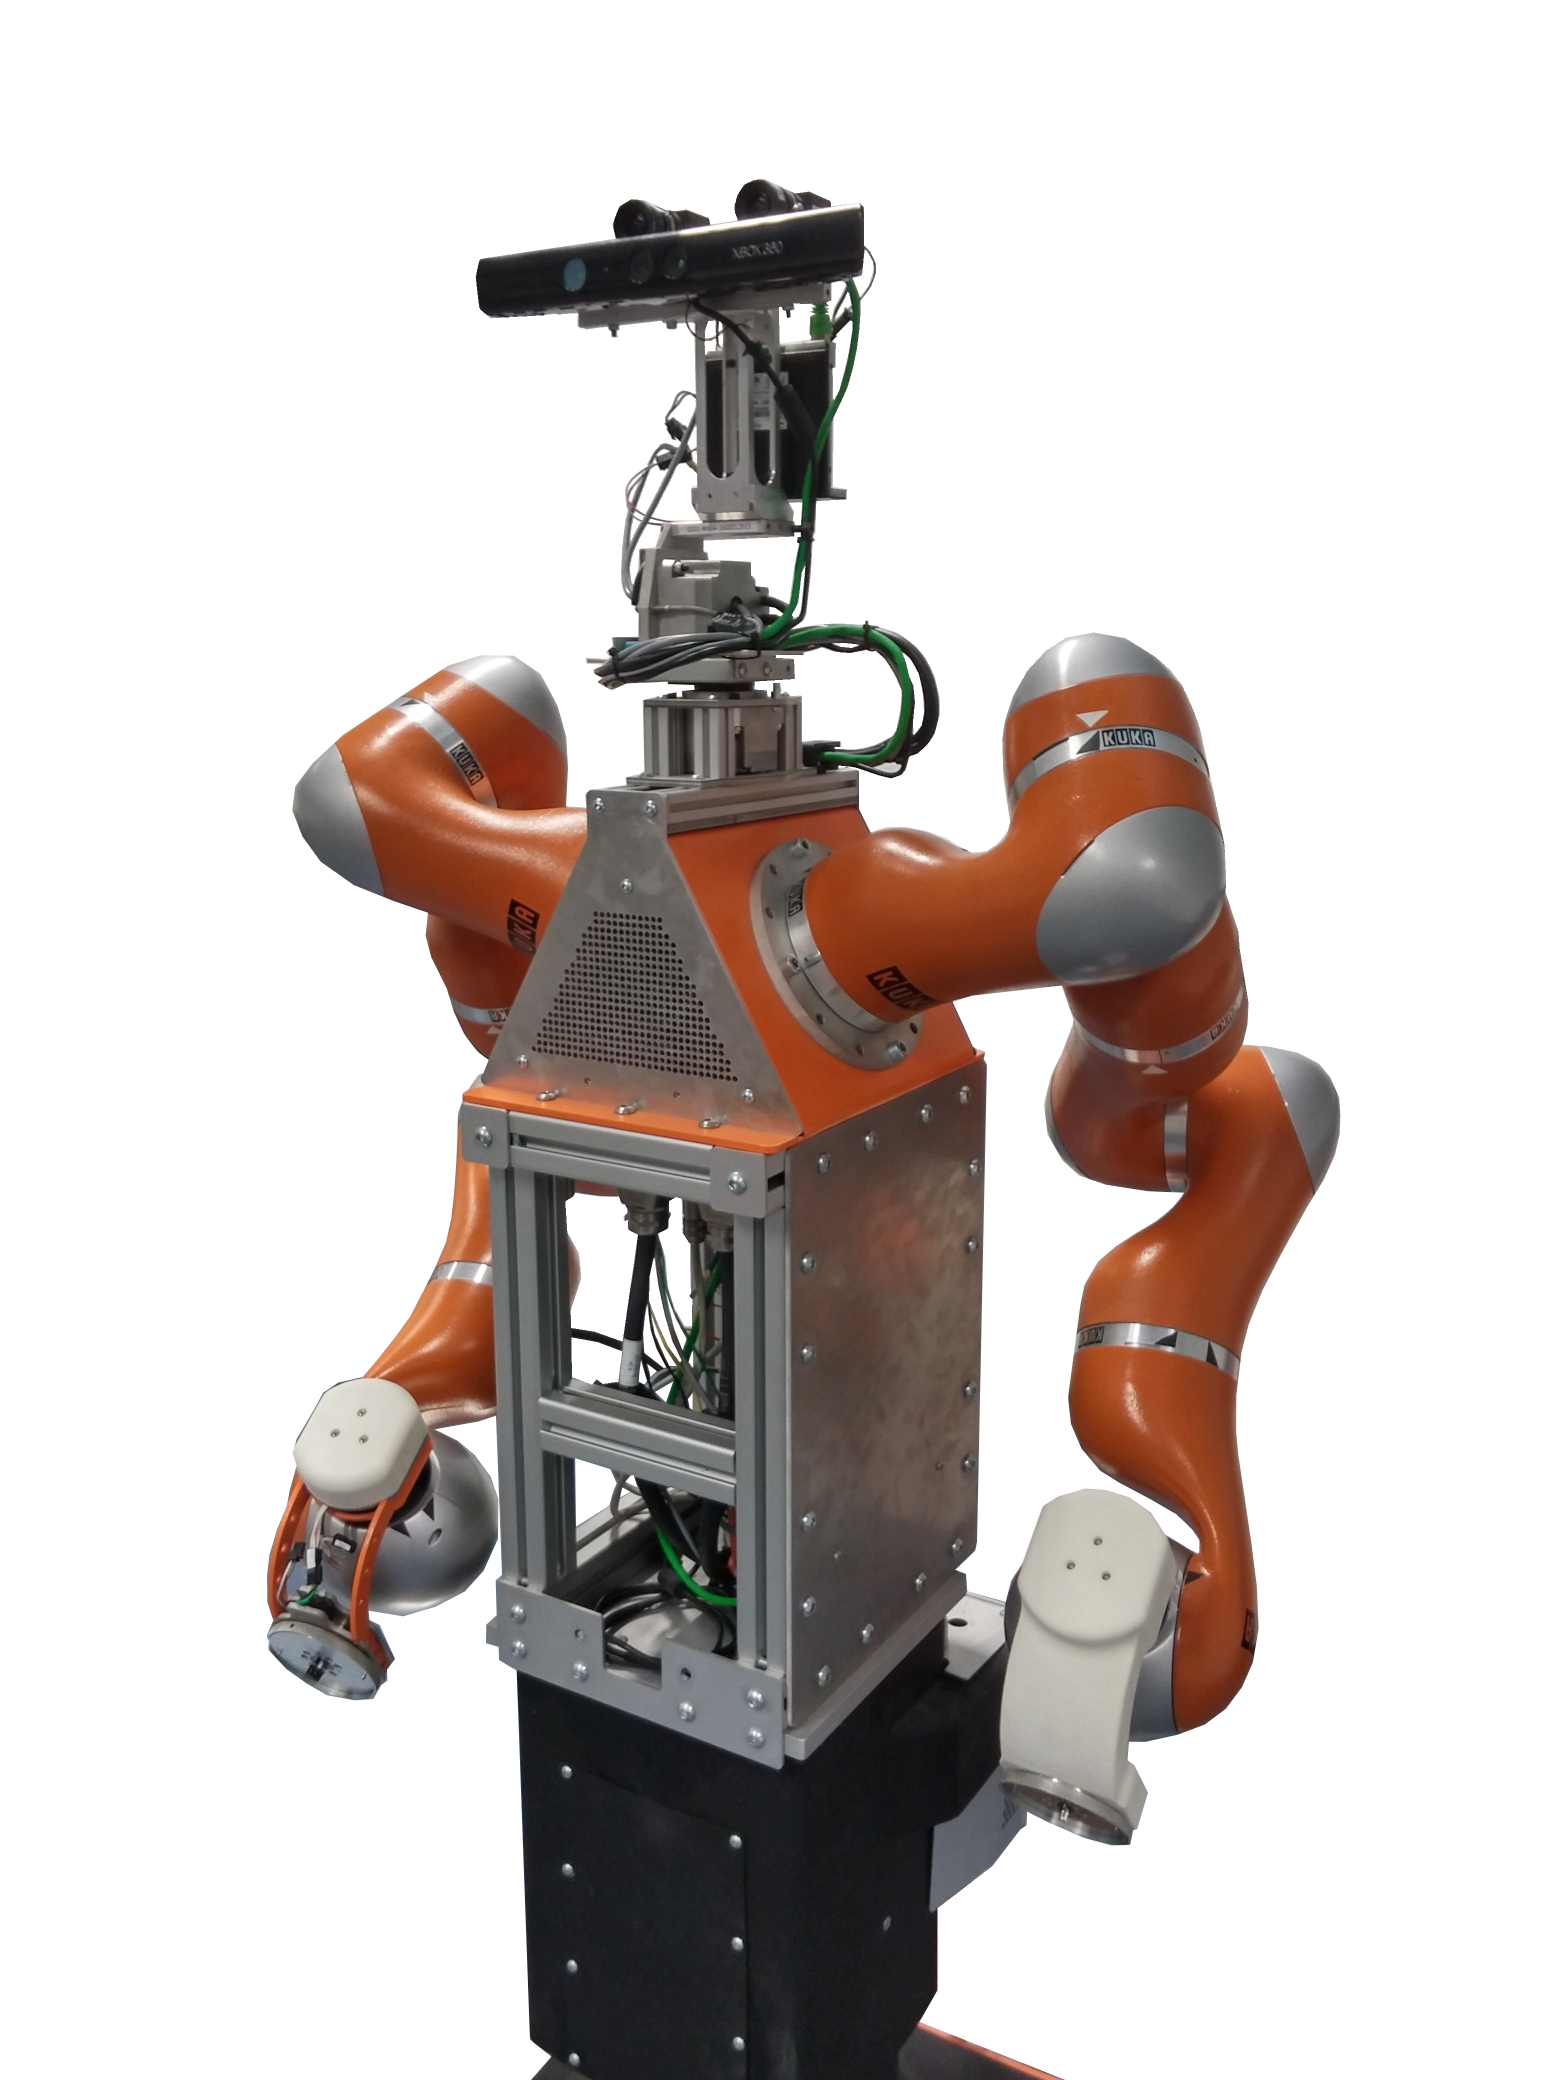
\includegraphics[width=0.5\textwidth]{graphics/velma.png}
\caption{Robot manipulacyjny Velma.}
\label{fig:velma}
\end{figure} 

Platforma jest niesymetrycznie podzielona na dwie niezależne części, przednią i tylną w sposób pokazany na rysunku \ref{fig:base_top}.
Przegub o jednym stopniu swobody (tzw. zawias) jest jedynym łącznikiem pomiędzy tymi dwoma fragmentami.
Zadaniem tego przegubu jest zmniejszanie wpływu nierówności podłoża na ruch bazy, aby każde koło dociskało do podłoża z taką samą siłą, jak po drugiej stronie osi.
Bez tego zawiasu nierówny teren uniemożliwiałby sprawne sterowanie platformą na skutek niedeterministycznego tarcia kół tej samej osi, powodując nieplanowany skręt.
Niedeterministyczne tarcie kół jest niewykrywalne w bezpośredni sposób, więc należy je wyeliminować na przykład za pomocą takiego przegubu.

Środki kół nie są rozmieszczone na wierzchołkach kwadratu. Jest 4 cm różnicy między szerokością, a długością.
Szerokość jest większa, co można zobaczyć porównując widok z prawej strony \ref{fig:base_side} z widokiem z tyłu \ref{fig:base_front}.
Dokładne wymiary są podane na rysunku \ref{fig:base_dims} i tabeli \ref{tab:dims}.

Platforma podatna jest na losowy ruch przy rozpoczynaniu jazdy i hamowaniu.
Jest to spowodowane tym, że asymetria rolek będzie nadawać kołom różne siły, a w związku z tym różne prędkości, co w efekcie może powodować niedeterministyczny ruch.
Należy także wziąć tutaj pod uwagę nieprzewidywalne opory, jak nierówne tarcie rolek o powierzchnię \cite{braking}.

\begin{figure}[H]
\centering
 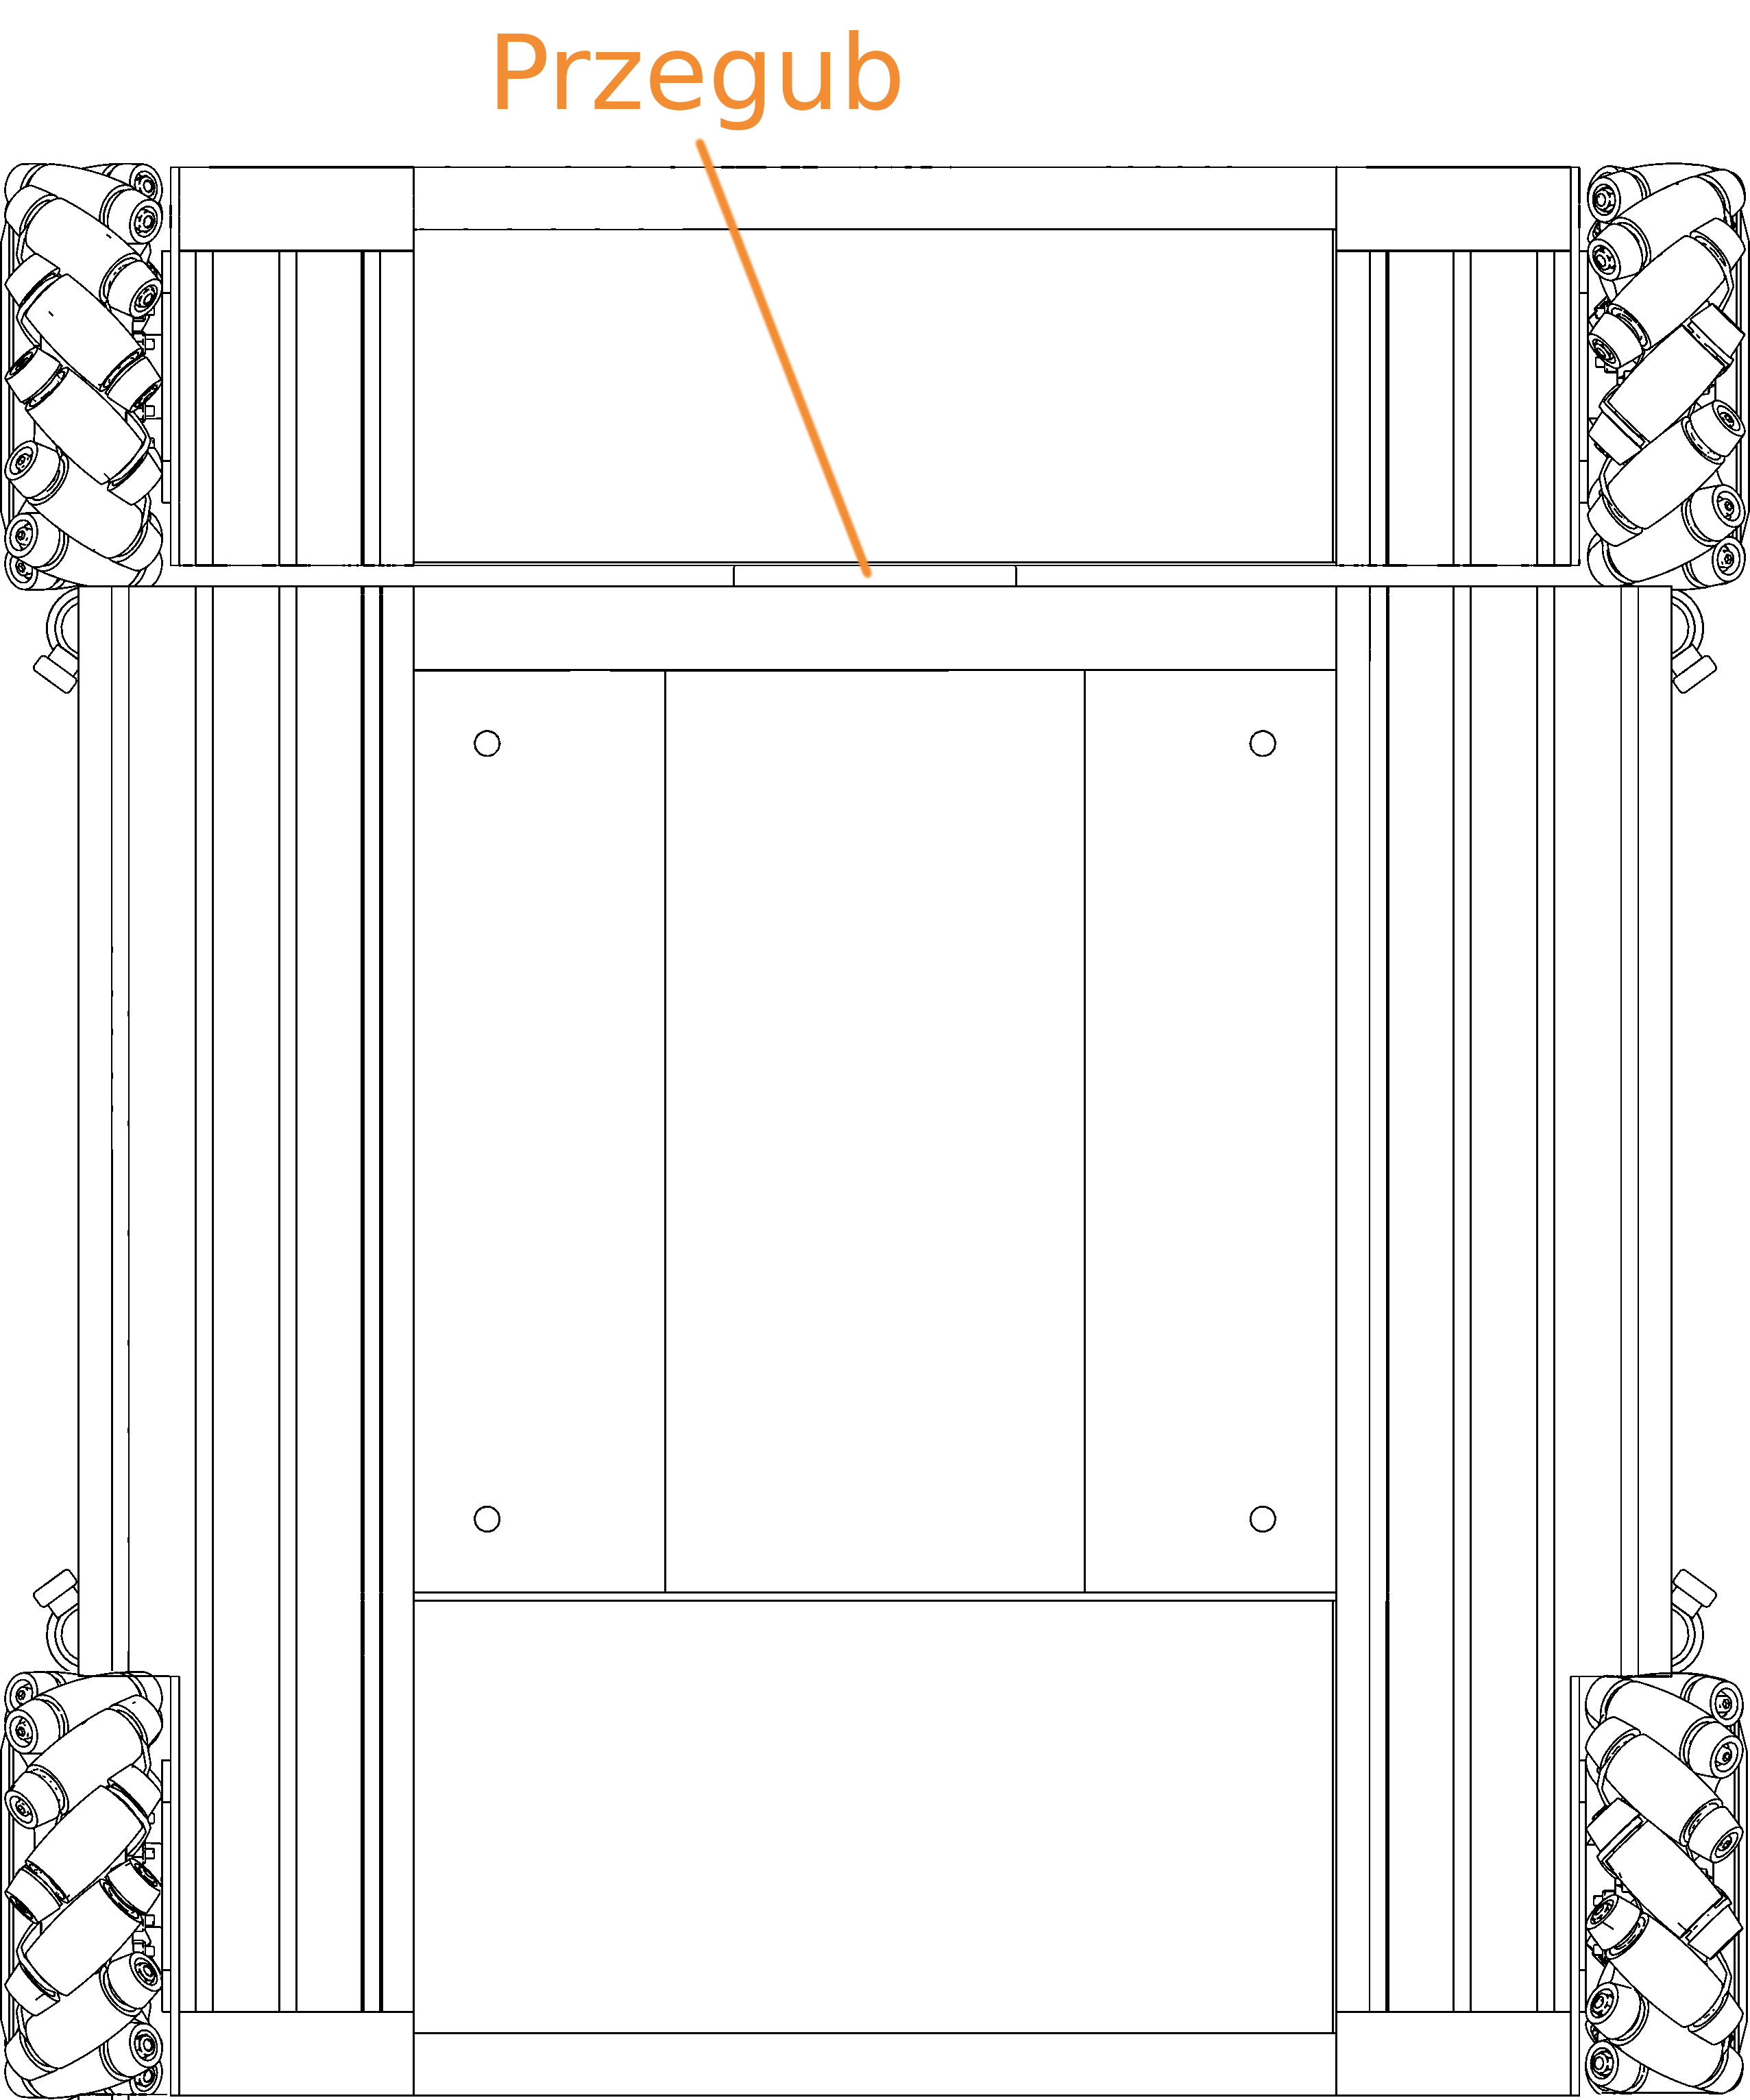
\includegraphics[width=0.5\textwidth]{graphics/base_top.png}
\caption{Platforma mobilna --- widok od góry. Przegub zawiasowy łączy dwie części.}
\label{fig:base_top}
\end{figure} 

\begin{figure}[H]
\centering
 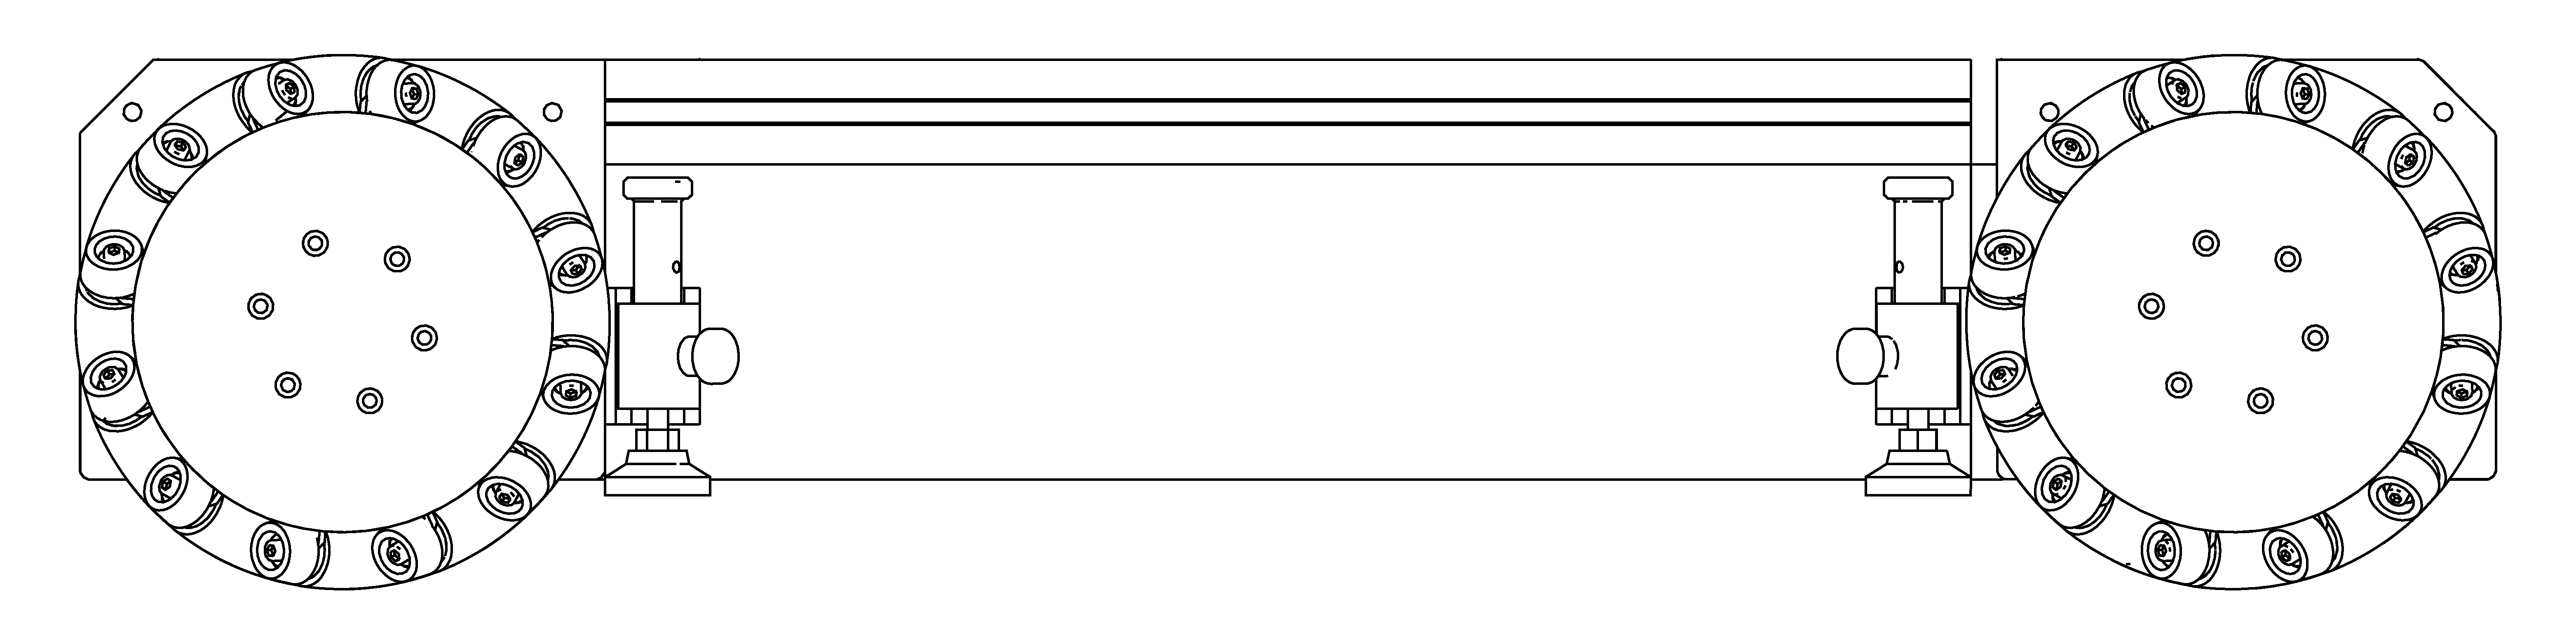
\includegraphics[width=0.5\textwidth]{graphics/base_side.pdf}
\caption{Platforma mobilna --- widok z prawej strony.}
\label{fig:base_side}
\end{figure} 

\begin{figure}[H]
\centering
 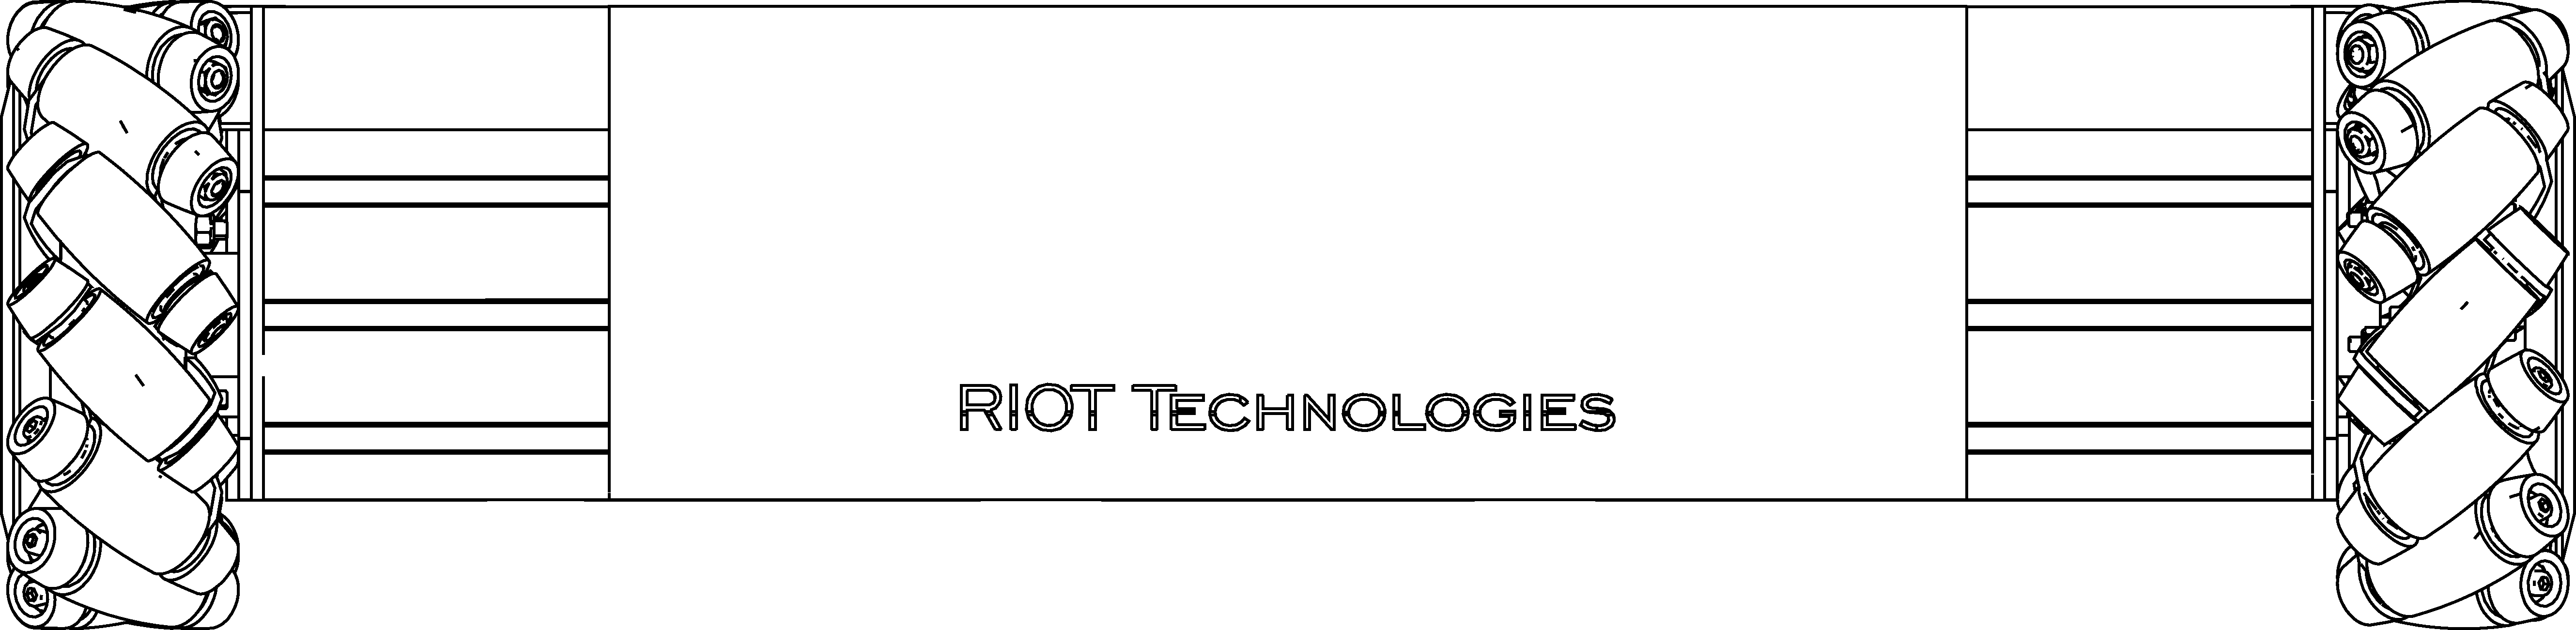
\includegraphics[width=0.5\textwidth]{graphics/base_front.pdf}
\caption{Platforma mobilna --- widok z tyłu.}
\label{fig:base_front}
\end{figure} 

Platforma posiada 3 stopnie swobody. Pierwszym i drugim jest ruch bez obrotu w osiach X i Y.
Trzecim stopniem jest dowolny obrót po płaszczyźnie podłoża.

\section{Koła szwedzkie}
Koła szwedzkie, zwane także kołami Mecanum, to specjalne koła z dodatkowymi rolkami na obwodzie ustawionymi pod kątem $45^\circ$ do osi koła.
Rolki są pasywne i obracają się niezależnie od siebie. Każde koło ma 12 takich rolek, patrz rysunek \ref{fig:wheel}.
Ich osie ustawione są w ten sposób, że osie rolek dwóch kół z tej samej strony robota przecinają się pod kątem prostym.
Innymi słowy, robot ma identycznie ustawione koła na przeciwległych wierzchołkach, i razem ustawione są w kształt litery \emph{X} patrząc na nie z góry.
Warto pamiętać, że oś aktualnie dolnej rolki jest prostopadła do osi górnej rolki.

Istnieje również odwrotna odmiana ustawienia kół, w której rolki tworzą literę \emph{O}, czyli oś przednia jest zamieniona z tylną, lub jakby cała platforma była odwrócona do góry nogami.
Ten drugi sposób także pozwala na ruch wielokierunkowy, ale nie jest tak często stosowany \cite{paletobot}.

\begin{figure}[H]
\centering
 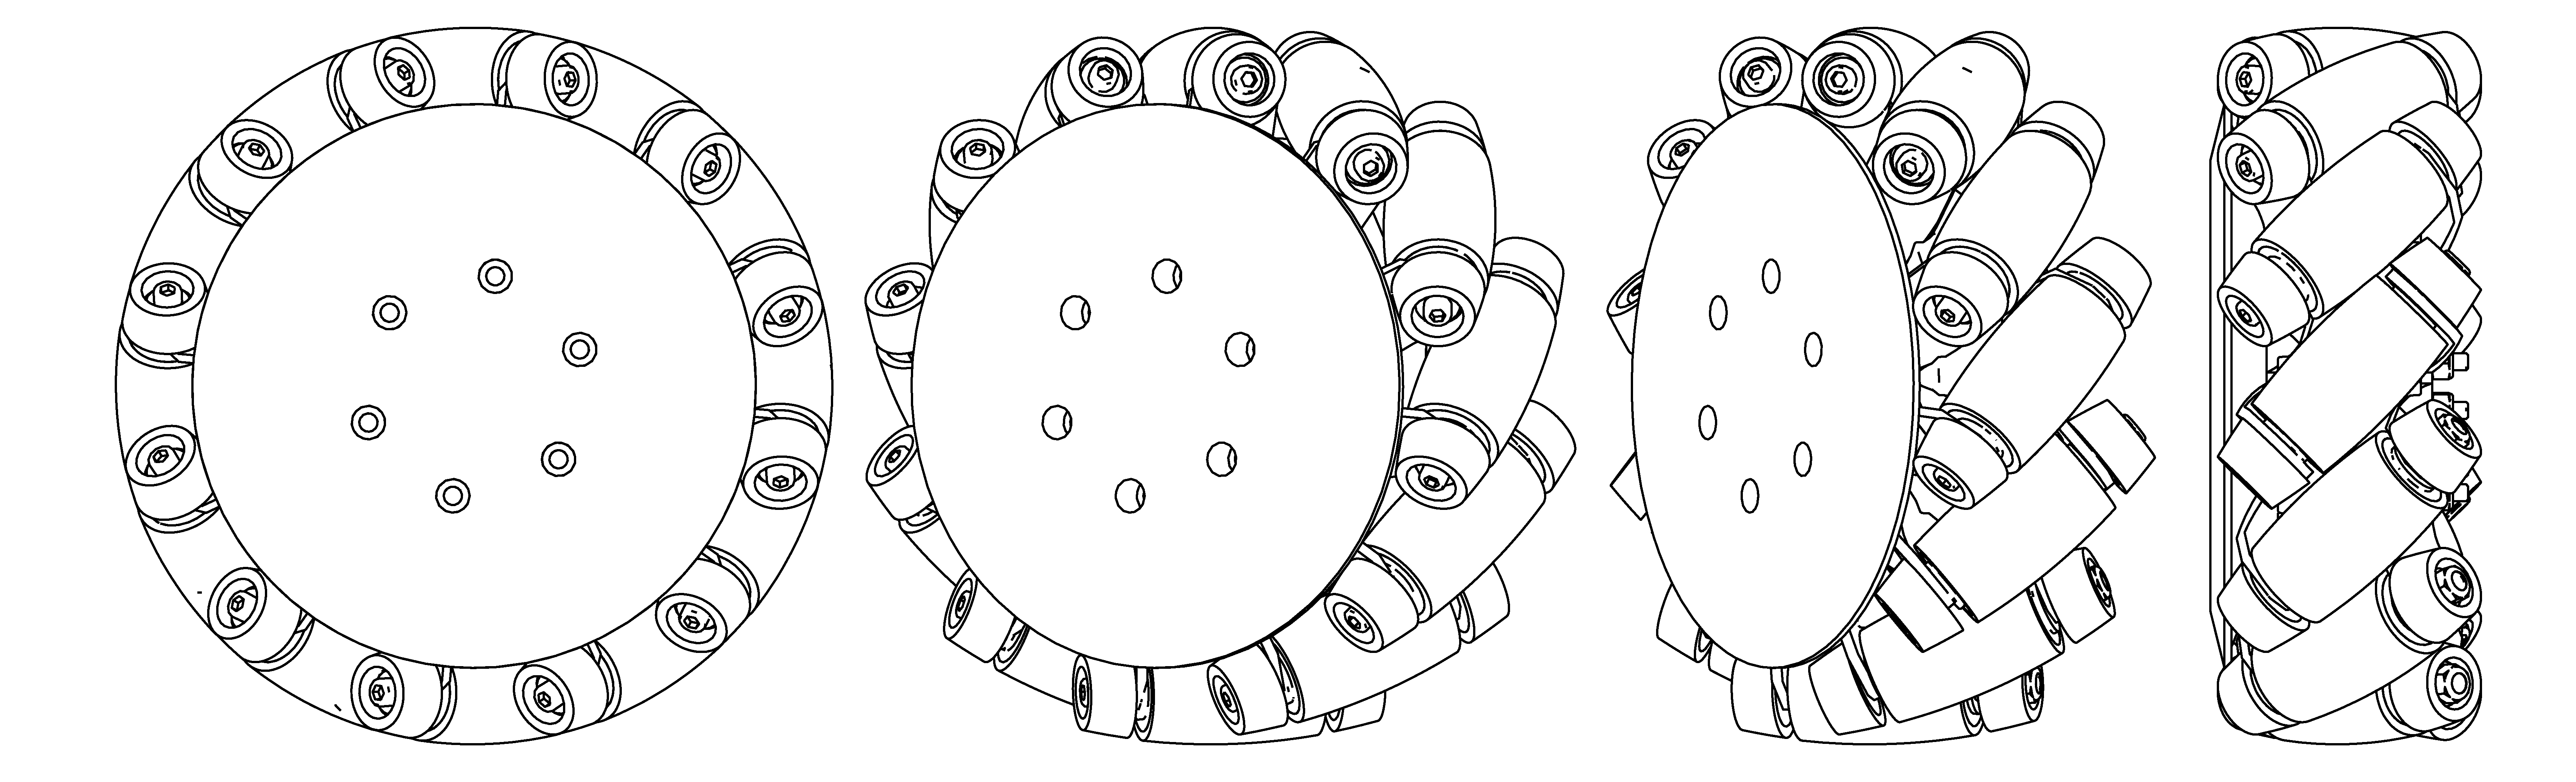
\includegraphics[width=\textwidth]{graphics/wheel.pdf}
\caption{Widok 12 rolkowego koła szwedzkiego opisywanej platformy wielokierunkowej.}
\label{fig:wheel}
\end{figure} 

Każde koło ma 3 stopnie swobody. Pierwszym jest obrót całego koła wzdłuż osi.
Drugim są rotacje pojedynczych rolek, a trzecim poślizg obrotowy w miejscu styku rolki z podłożem \cite{kinematic_modeling}.

Na podstawie rysunku \ref{fig:wheel} widać, że krzywizna rolki jest tak ustawiona, aby punkt kontaktu rolki z podłożem płynnie przechodził na następną rolkę w trakcie obrotu.
Celem jest utrzymanie równej odległości osi od płaszczyzny podłoża.
Nie powinno być efektu przeskoku z jednej rolki na drugą, gdyż to wprowadza nierówne tarcie, losowe poślizgi i nadmierne zużycie elementów wykonawczych.
Pojedyncza rolka zawiera się w paraboloidzie, wzory opisujące kształt rolki są złożone.
Zazwyczaj przybliża się ją torusem w celu uproszczenia produkcji \cite{rollers}.

Istnieją także inne budowy kół, złożone z wielu małych rolek tak, aby w każdym momencie kilka rolek dotykało podłoża.
Można także złożyć kilka powyższych kół obok siebie w jednym kole.
Przydatne jest to dla robotów transportujących duże masy, gdyż zmniejsza to obciążenie pojedynczych rolek.
Niestety taka budowa jest chroniona aktywnym patentem, więc pojedyncze koło, na które patent już wygasł z jest jedynym popularnie używanym \cite{paletobot}.

Podstawowym problemem technologicznym koła jest skomplikowana budowa, ale także ślizganie się rolek po powierzchni.
Odległość osi od płaszczyzny nieznacznie zmienia się przy przenoszeniu ciężaru z rolki na rolkę, co przy dużych prędkościach powoduje drgania i jeszcze większe błędy pomiarów.
Środkowy przegub zmniejsza ich przenoszenie na drugą część platformy.
Poślizg kół powoduje, że enkodery nie mogą być jedynymi czujnikami służącymi do wyznaczania pozycji bazy, gdyż są zbyt mało dokładne \cite{heavy}.

\section{Czujnik laserowy}
Platforma wyposażona jest w dwa czujniki laserowe firmy SICK.


\section{Składniki systemu}
Środowisko symulacyjne składa się z kilku odrębnych modułów, które komunikują się ze sobą poprzez specjalne interfejsy wykorzystujące kolejki wiadomości.
Taka implementacja komunikacji pozwala zmieniać i reimplementować poszczególne elementy i używać różnych języków programowania zachowując tę samą komunikację między składnikami nie tracąc kompatybilności między sobą.
Możliwe jest także przesyłanie wiadomości przez sieć, co pozwala na rozproszenie systemu.

%TODO Zmienić na Tikz
\begin{figure}[H]
\centering
 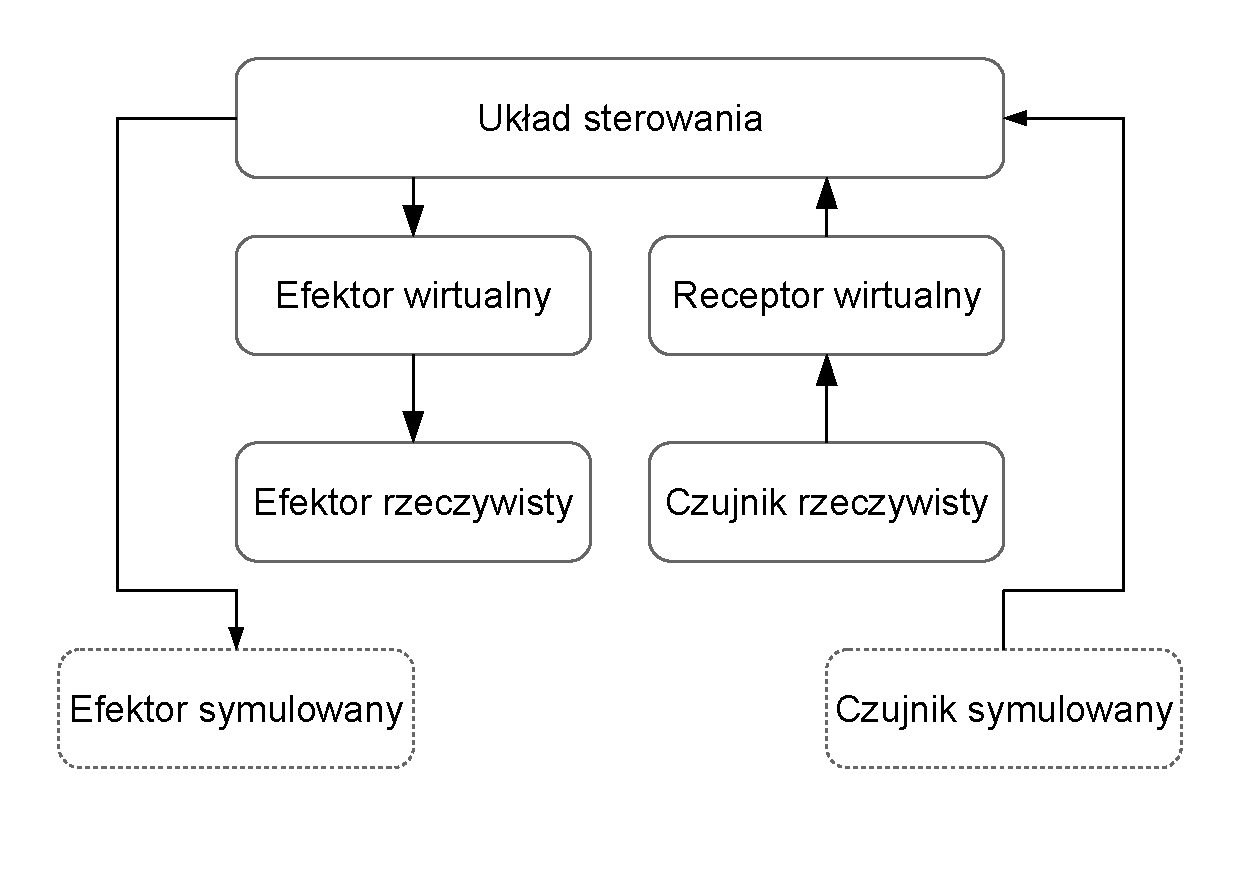
\includegraphics[width=0.8\textwidth]{graphics/agent.pdf}
\caption{Struktura agenta upostaciowionego.}
\label{fig:agent}
\end{figure} 

Można to przedstawić za pomocą zapisu agentowego, jak na rysunku \ref{fig:agent}.
Agent upostaciowiony składa się wilku modułów komunikujących się ze sobą za pomocą różnych systemów.

Nadrzędnym modułem jest układ sterowania, który na podstawie odczytów z czujników generuje sterowanie dla efektorów.
Ważne jest, aby komunikacja z rzeczywistymi urządzeniami była identyczna, jak z ich modelami, dzięki czemu taki system będzie przenośny i niezależny.

Efektor rzeczywisty, na przykład serwomotor, jest sterowany za pomocą efektora wirtualnego, który zamienia wyjście układu sterowania na sygnały sterujące dla silnika napędowego.
Przykładowo zmienia podaną liczbę oznaczającą zadaną prędkość na odpowiednie napięcie na wyjściu.

Zamodelowany efektor symulowany również przyjmuje te same sygnały do układu sterowania, lecz nie zamienia ich na sygnały sterujące, a wywołuje odpowiednie funkcje maszyny symulacyjnej nadające siły i prędkości obiektom w przestrzeni wirtualnej.

Receptor wirtualny pobiera surowe dane z czujnika, przekształca na odpowiedni format, usuwa błędy i szum tak, aby program sterujący mógł wykorzystać te dane w prosty sposób. 
Doskonałym przykładem jest tutaj kamera Kinect, w której to zachodzi odczytanie obrazu z kilku kamer.
Następnie obraz przesyłany jest do komputera w którym sterowniki interpretują dane usuwając błędy, tworzą mapę głębokości, wykrywają szkielety i sylwetki osób.
Te dane mogą być wykorzystane łatwo w grach i programach sterujących.

Modelowanie receptora, tak jak w przypadku efektora polega na wygenerowaniu odpowiednich danych używając odpowiednich funkcji w przestrzeni wirtualnej.
Mogą one polegać na puszczaniu promieni symulujących laser, lub wręcz renderowaniu obiektów, aby uzyskać obraz z wirtualnej kamery.
Receptor symulowany ma pełną wiedzę o symulowanym świecie, dokładne pozycje i prędkości wszystkich obiektów, dane o kolizjach itp. 
Pozwala to na łatwe symulowanie receptorów nie mogących mieć odwzorowania w rzeczywistości, co przydatne jest w pierwszych stadiach testowania i wyznaczaniu statystyk.

\subsection{Model 3D}
Model 3D bazy mobilnej opisany równaniami matematycznymi powinien mieć zachowanie najbardziej jak to tylko możliwe zbliżone do oryginału.
Musi uwzględniać masy i momenty bezwładności elementów składowych, a także wszystkie tarcia.
Model obejmuje więzy na ruchome elementy, takie jak koła i rolki, aby umożliwić symulację przegubów.

Model składa się z elementów odwzorowujących rzeczywiste części składowe bazy mobilnej.
Elementy posiadają takie cechy, jak pozycja w modelu, masa, moment bezwładności, kształt, materiał fizyczny i wygląd.
Dodatkowo należy uwzględnić więzy tych składowych w postaci symulowanych przegubów.
W przypadku tej bazy istnieje jeden typ więzów o jednym stopniu swobody (zawias).
Więzy mogą oddziaływać siłą na elementy do których są podłączone symulując silniki.

Elementy składowe i symulowane przeguby oddziałują bezpośrednio z maszyną do symulacji fizycznej. 
To kształt, masy i momenty bezwładności brył są argumentami funkcji liczących.
Maszyna symulacyjna oblicza odpowiednie prędkości i nadaje podanym obiektom w podobny sposób, jak ma to miejsce w rzeczywistości.

Do modelu doczepia się wirtualne czujniki generujące odpowiednie dane na podstawie symulacji i rozkładu losowego.
Nie są to pełne dane o stanie modelu, jakie posiada maszyna do symulacji, gdyż czujniki fizyczne również nigdy nie mają pełnej informacji o stanie urządzenia.
Należy dodać losowy szum i błędy, aby przybliżyć ich zachowanie do rzeczywistych czujników.

Dla ozdoby można wykorzystać istniejący model CAD do stworzenia siatki trójwymiarowej i nadania symulowanemu obiektowi wyglądu zbliżonego do fizycznego robota.

 \subsection{Sterownik silników}
Program sterujący generuje abstrakcyjne dane, na przykład liczbę zapisaną binarnie.
Przykładowy silnik fizyczny nie jest w stanie działać na ich podstawie, on potrzebuje odpowiedniego napięcia na wejściu.
Do tłumaczenia jednych danych na drugie potrzebny jest sterownik niskopoziomowy.
Najczęściej implementowany jest w formie mikrokontrolera, lub podobnego systemu wbudowanego.

Jego zadanie to odczytanie danych podanych przez program sterujący i na przykład generowanie na ich podstawie odpowiedniej fali PWC, lub obsługa przetwornika cyfrowo-analogowego.
Do innych zadań może należeć kontrola, czy żądana wartość nie uszkodzi urządzenia.
Zazwyczaj sterownik może komunikować się z powrotem z resztą systemu, aby zgłaszać ewentualne awarie.

Taki program i powiązany z nim układ elektroniczny są najczęściej dostarczone przez producenta robota i nieznane użytkownikowi.
Dodatkowo tworzy kolejną warstwę abstrakcyjną dla sterownika głównego, który nie musi zważać na generowanie różnych danych dla różnych modeli tych samych efektorów.
 
W środowisku wirtualnym należy stworzyć moduł o podobnym działaniu.
Powinien przyjmować dane w dokładnie takim samym formacie, jak opisany wyżej układ, aby był łatwo wymienialny na sterownik fizycznego urządzenia bez ingerencji w główny program sterujący.
Zamiast zamieniać odczytane dane na analogowe wartości, on wywołuje odpowiednie funkcje maszyny symulacyjnej, aby wywołać taki sam efekt, co na rzeczywistym efektorze, lecz w wirtualnej przestrzeni symulacji.
Jako argumenty podaje parametry fizyczne symulowanego obiektu, oraz przyłożone siły.
 

\subsection{Sterownik czujników}
Implementowany podobnie do sterownika silników ma za zadanie konwertować surowe i obarczone błędami dane z czujników na format zrozumiały dla programu sterującego.
W tym miejscu usuwa się błędy grube, niweluje stałe na podstawie kalibracji, wygładza szum i interpretuje dane, aby pozyskać wymagane przez wyższe warstwy informacje.

Przykładowo czujniki laserowe zwracają jedynie ciąg pomiarów, ale to do tego programu należy interpretacja wykrytych kształtów, łączenie punktów i obróbka do formatu zrozumiałego dla wyższych podzespołów.
Większość zaawansowanych receptorów posiada owe układy cyfrowe i programy wbudowane w urządzenie.
Dostarczone przez producenta tak samo, jak sterowniki efektorów.
 
Symulując ten element budujemy program generujący dane na podstawie aktualnego stanu maszyny do symulacji w sposób, w jaki działa czujnik w rzeczywistości.
Na przykład dla czujnika laserowego wypuszczamy setki promieni i obliczamy ich punkty przecięcia się z wirtualnymi modelami.
Możemy renderować obraz, aby symulować kamerę.

Ponieważ dane fizyczne nigdy nie są idealne, w celu przybliżenia wyjścia wirtualnego czujnika do oryginału, dodajemy szum o odpowiednim rozkładzie i błędy.

\subsection{Program sterujący}
Cześć odpowiedzialna za logikę aplikacji. Tutaj obliczane jest sterowanie na podstawie dostarczonych odczytów z czujników.
Zazwyczaj wykorzystuje się tu dużą ilość bibliotek dostarczających zaawansowane algorytmy.
Ich zadania mogą polegać na budowie wewnętrznej mapy, wyznaczaniu ścieżki, omijaniu przeszkód, odwrotnej kinematyce i tym podobnych.

Taki program zwykle działa na mocniejszych układach, niż sterowniki ze względu na duże zapotrzebowania na moc obliczeniową.
Jeśli robot komunikuje się z użytkownikiem, lub zwraca dane, to zachodzi to w tym module. 

Programy sterujące mogą być implementowane w językach wysokopoziomowych, nawet skryptowych, gdyż wymagania czasowe nie są rygorystyczne.
Co więcej, często się zdarza, że odpowiednie składowe programu bazują na różnych technologiach.

Środowisko symulacyjne powinno zapewnić pełną abstrakcję komunikacji tego modułu.
Oznacza to, że niezależnie, czy program działa na rzeczywistym robocie, czy symulacji wirtualnej, zawsze powinien móc komunikować się i otrzymywać dane w tym samym formacie.
W idealnym świecie program nie powinien mieć możliwości stwierdzić, czy steruje symulacją, czy oryginałem.

\section{Technologie}
Symulator daje użytkownikowi do dyspozycji odpowiednią maszynę symulacyjną odpowiedzialna za obliczenia fizyczne, a także API do obsługi całej symulacji.
Zaawansowana maszyna symulacyjna powinna dobrze obsługiwać tarcia, więzy na ruch obiektów, przyłożone siły, materiały fizyczne dla określania tarcia i sprężystości, 
oraz wszystko to, co potrzebne do jak najwierniejszego odtworzenia zachowania rzeczywistego obiektu.

Na rynku jest wiele różnych maszyn zarówno do symulacji w czasie rzeczywistym, jak i do wyznaczania pozycji obiektów po długich obliczeniach.
Jedne z technologii są otwartoźródłowe, inne nie. Mogą używać tylko procesora, lub też być wspomagane przez kartę graficzną.
Niektóre prócz zderzeń obiektów potrafią także symulować rozpływ cieczy, dymy, płótna, ciała sprężyste i strukturę wewnętrzną obiektów, lecz te funkcjonalności nie są potrzebne dla naszej symulacji.

\subsection{Gazebo}
Program do pobrania z \cite{gazebo_website}. Ten symulator graficzny jest dość prosty w obsłudze, skupia się na symulowaniu podanych danych, a mniej na możliwości ich łatwego przygotowania.
Zazwyczaj używany w trybie wsadowym, uruchamiany z argumentami z linii poleceń i plikiem \emph{world} opisującym symulację.
Plik ten zawiera nazwy i ścieżki innych umieszczanych modeli i wtyczek.
Z tego powodu interfejs graficzny jest dość ubogi.

Program przeprowadza symulację podanych modeli używając jednego z czterech popularnych maszyn symulacyjnych: ODE, Bullet, Simbody lub DART.
Wszystkie te projekty są wolnym oprogramowaniem i używane są także w innych programach, jak Blender.

Symulator oprócz tego ma wbudowany edytor modeli w którym możemy składać odpowiednie obiekty od razu w przestrzeni trójwymiarowej.
Edytor budynków pozwala na stawianie wirtualnych ścian, korytarzy, drzwi i ogólnego otoczenia w którym roboty mogą pracować i być symulowane.
Jakość wykonania tych składników pozostawia wiele do życzenia, brak jest tak podstawowych funkcji, jak cofanie ruchu.
Dlatego lepiej jest definiować model we wczytywanym pliku tekstowym.
Również tworząc modele poza edytorem w ten sposób mamy nad nimi pełną kontrolę, a parametry można ustawiać z dowolną dokładnością.

Gazebo przyjmuje modele w specjalnym formacie SDF. Jest to ustandaryzowany, zdefiniowany zewnętrznie format do opisywania składników robotów i czujników.
Dzięki temu taki plik może być użyty także gdzie indziej, pod warunkiem przestrzegania standardu.
Składnia jest zwykłym plikiem XML, co znaczy, że może być on tworzony na każdym edytorze tekstowym.

Wtyczka do sterowania modelem jest skompilowaną biblioteką dołączaną na starcie programu.
Tworzy się ją w C++ jako klasę dziedziczącą po abstrakcyjnej klasie dostarczonej przez Gazebo.
Dzięki temu może się komunikować z innymi systemami poprzez dowolne mechanizmy, nawet systemowe, jak gniazda, czy pamięć współdzielona.
Jednak Gazebo dostarcza także swój własny mechanizm kolejek wiadomości, który sprawdza się w jednolitej komunikacji z innymi programami.

Program jest wspierany na systemie Ubuntu ale bez problemu można go także skompilować pod inne systemy.
Interfejs jest dopracowany i przestrzega wielu ustawień systemowych, jak DPI.
Uruchamianie jest proste i nie wymaga dodatkowych ustawień, uruchamiania skryptów inicjalizujących, tworzenia odpowiednich katalogów, czy definiowania zmiennych systemowych.
Standardowo, jak inne programy tworzy ukryty katalog w katalogu domowym użytkownika, gdzie znajdują się wszystkie modele i logi.
Czasami trzeba używać tego katalogu, aby umieścić tam swoje modele, które Gazebo będzie automatycznie umieszczał w symulacji.

Gazebo jest składnikiem systemu ROS, kod źródłowy jest dzielony w ramach wspólnej organizacji, chociaż różne osoby odpowiadają za rozwój tych oprogramowań.
Kolejne wersje Gazebo są powiązane z wersjami ROSa, nie można użyć przestarzałej wersji Gazebo z nowszym ROSem i odwrotnie.
Symulator można zainstalować osobno, lub jako jeden z pakietów ROSa.

\subsection{V-Rep}
Program do pobrania z \cite{vrep_website}. Duże i skomplikowane środowisko reklamujące się wieloma zaawansowanymi mechanizmami i funkcjami.
Pomimo otwartego kodu, użycie komercyjne jest płatne. Dla zastosowań akademickich program jest rozdawany bez opłat.
Bogaty interfejs graficzny zakłada budowę i symulację wszystkiego w tym jednym programie.

Używa dwóch z maszyn symulacyjnych, co Gazebo, czyli ODE i Bullet, oraz dodatkowo Vortex i Newton. Z tej czwórki tylko Vortex ma zamknięty kod.

Problemem jest także zapisywanie utworzonych w systemie modeli.
Program tworzy drzewiastą strukturę modelu w pliku binarnym własnego formatu, co uniemożliwia edycję i oglądanie modelu bez posiadania całego programu i importowania modelu do symulacji.
Brak przenośności, czy wsparcia systemu kontroli wersji dla takich zbiorów bajtów także jest problemem.

Pisanie wtyczek najczęściej odbywa się w C. Są też jednak dostępne inne języki skryptowe, jak Lua, Matlab, Java itp.
Komunikacja z innymi programami odbywa się poprzez specjalne dodatki do środowiska.
API pozwala nam stworzyć mały, wbudowany interfejs graficzny do sterowania symulacją poprzez przyciski i suwaki.

Ze strony producenta pobieramy gotowe archiwum z programem, który nie wymaga żadnej instalacji i posiada wszystkie potrzebne zasoby do pracy i nauki, jak przykładowe modele istniejących komercyjnych robotów.
Program działa w trzech najpopularniejszych systemach operacyjnych --- Windows, Linux i OS X.

\subsection{ROS}
Platforma programistyczna do pobrania z \cite{ros_website}.
ROS jest skrótem od \emph{Robot Operating System}, lecz jego nazwa jest bardzo myląca.
Nie jest to żaden system operacyjny, lecz obszerna platforma programistyczna (framework) zawierająca odpowiednie biblioteki i narzędzia do tworzenia programów sterujących.
ROS stara się w łatwy sposób dostarczyć wszystko, co potrzebne do budowy logiki aplikacji sterowania.
Są tu algorytmy wyznaczania tras, budowy map, manipulowania itp. 

Twórcy zachęcają, aby uzupełniać brakujące moduły swoimi własnymi, a potem dzielić się nimi z resztą programistów, aby każdy mógł skorzystać, jeśli ma podobny problem.

Programy dla ROS pisze się w C++, lub Pythonie i integruje z robotem za pomocą kilku gotowych struktur kolejek wiadomości.
Platforma ta także posiada moduły do wizualizacji odbieranych danych w formie graficznej.
Nie jest to symulator, gdyż sam nie generuje żadnych danych, a jedynie prezentuje gotowe.

Działanie systemu jest oparte o pakiety. Każdy pakiet jest katalogiem zawierającym w sobie pliki opisujące jego parametry i skrypty używane w kompilacji.
Pakietem może być wszystko, od modelu do programu pomocniczego.
Pakiety mogą być zależne od siebie, ale nigdy nie wskazują nawzajem swoich bezpośrednich ścieżek.

Na przykład jeden pakiet wymaga pliku nagłówkowego generowanego przez kompilację drugiego pakietu, ale załącza go w kodzie tak, jakby był systemowy.
Globalny skrypt kompilacji ROSa dba o odpowiednie podawanie ścieżek, kolejność kompilacji programów i załączanie nazw.

Komunikacja między programami odbywa się w sposób ciągły przez kolejki wiadomości, lub pojedyncze asynchroniczne wywołania zwracające wynik.
Program może nadawać strumień wiadomości, ale nie koniecznie musi istnieć w tym czasie odbiornik.
Można buforować wiadomości, podglądać strumienie, tworzyć wykresy z danych, podłączać nadajnik do kilku odbiorników, podglądać graf zależności itp.
Do wszystkiego służy bogaty zestaw komend.

Instalacja programu na systemie operacyjnym jest dużym problemem.
Z wyjątkiem odpowiednich wersji Ubuntu nie ma łatwego sposobu na wgranie go do innych systemów.
Na przeszkodzie stoją błędy kompilacji dla nowszych wersji kompilatorów i inne problemy w czasie wykonywania wykonania, jak naruszenie ochrony pamięci. 
Instalacja alternatywnych pakietów i ręczna kompilacja niektórych części nie działa we wszystkich przypadkach.
Głównym problemem jest niezgodność wersji zewnętrznych bibliotek.

Rozwiązaniem tego problemu jest instalacja tej platformy programistycznej na maszynie wirtualnej, lub na systemie uruchamianym z dysku zewnętrznego. 
Takie rozwiązanie także daje dostęp do najnowszej wersji ROS \emph{Kinetic Kame} z końca maja 2016 roku.

Uruchomienie platformy programistycznej na systemie wymaga wielu dodatkowych komend inicjalizujących, a także dopisywania do tworzonych projektów licznych plików konfiguracyjnych za pomocą dostarczonych skryptów.
Używanie modułów z linii poleceń wymaga ustawienia kilku zmiennych systemowych poprzez wczytywania całościowych plików.
Użycie niektórych funkcji ROS wymaga uruchomionego demona serwera w tle.

Ogólnie instalacja i używanie ROS na systemie zostawia dużo różnorodnych plików, dlatego lepiej jest trzymać ją z dala od codziennego systemu operacyjnego, na maszynie wirtualnej, lub dysku.
Z drugiej jednak strony wirtualizacja systemu operacyjnego z ROS bardzo ogranicza dostępną moc obliczeniową potrzebną takim programom w dużych ilościach.

\subsection{Narzędzia}
Do tworzenia oprogramowania na systemach Unixowych można użyć dowolnych edytorów, gdyż standardowo wszystko jest potem kompilowane za pomocą narzędzi wiersza poleceń i skryptów.
Jednak warto sobie ułatwić pracę zaawansowanymi środowiskami graficznymi.
\begin{description}
 \item[Gazebo] będzie użyty do symulacji z jego domyślną maszyną symulacji fizyki ODE.
 \item[ROS] użyty zostanie jako gówna platforma programistyczna. Pod łatwą komunikację z jego modułami należy budować sterowniki wirtualne.
 \item[Atom] jest popularnym uniwersalnym edytorem tekstowym. Dzięki rozszerzaniu przez wtyczki dobrze się sprawdza przy obróbce plików XML i skryptów.
 Będzie użyty do konstrukcji modelu.
 \item[CMake] to popularny i polecany przez ROS i Gazebo system budowy kodu. Program tworzy na podstawie swoich plików konfiguracyjnych plik \texttt{makefile} do kompilacji źródeł i łączenia bibliotek.
 \item[GCC] będzie użyty do kompilacji, gdyż jest to najpopularniejszy tego typu program używany w GNU/Linux. Same symulatory zostały w nim skompilowane.
 Razem z nim użyty zostanie debugger GDB. 
 \item[Code::Blocks lub Eclipse] nadają się do pisania kompilowalnego kodu wtyczek. Można podłączyć je pod komendę \texttt{make} i korzystać z mechanizmów interpretacji błędnych wierszy, graficznego debugowania i podobnych.
 \item[Bash] będący bardzo popularnym językiem skryptowym nadaje się do automatyzacji pracy i uruchamiania wielu programów w kontrolowany i szybki sposób.
 Uniwersalne narzędzie pomagające w różnych miejscach.
 \item[Git] jest narzędziem kontroli wersji, które jest wskazane w każdym projekcie informatycznym. Kod należy dla bezpieczeństwa umieszczać także w usłudze GitHub.
 \item[Virtualbox] do ewentualnej wirtualizacji systemu operacyjnego z ROS, lub uruchomienie osobnego systemu z dysku zewnętrznego.
\end{description}

\section{Plan pracy}
\begin{enumerate}
 \item Należy stworzyć model w SDF zachowując wszystkie rozmiary i momenty rzeczywistej wersji.
Bryły składowe modelu muszą przypominać kształtem części z których składa się robot, należy im także ustawić parametry fizyczne, jak masę, moment bezwładności, materiał itp.

\item Zamodelować wszystkie więzy na koła, rolki i przegub, aby maszyna symulacyjna poprawnie symulowała obiekt.
Taki model powinien na tym stanie poprawnie reagować na wirtualne siły, lecz jego efektory nie będą jeszcze aktywne.
Można go prosto pobieżnie przetestować działając siłą na elementy i patrząc, czy reagują w spodziewany sposób.

\item Zapisanie wtyczki sterującej w Gazebo odczytującej odpowiednie dane z zewnątrz i wywołującej funkcje maszyny symulacyjnej, aby modyfikować ruch modelu.
Na tym poziomie można dobudować zamiennik programu sterującego jedynie do podawania prostych wartości bez odczytywania pomiarów i sterowania.

\item Zaprogramowanie wtyczki symulującej czujniki, aby generowały dane z enkoderów, oraz innych urządzeń, dodawały błędy pomiarowe, a następnie przekształcały dane na format zrozumiały dla programu sterującego.
Czujniki nie muszą być istniejące, mogą generować dane, jak pozycja i rotacja bardzo trudne do uzyskania rzeczywistymi czujnikami.

\item Wystawienie do zmiany w czasie rzeczywistym masy, momentu bezwładności, współczynników tarcia, aby pozwolić na proste testowanie działania systemu z różnymi współczynnikami.

\item Elementy pomagające w symulacji, jak model kinematyczny sterowany funkcją matematyczną i podłoże ze zmiennym współczynnikiem tarcia.

\item Programy pomocnicze zbierające i wyświetlające dane, interfejs graficzny.

\item Program sterujący w ROS. Największy i najbardziej skomplikowany element, na szczęście wspólny dla obu bytów --- wirtualnego i rzeczywistego.
Zazwyczaj nie jest to praca jednego człowieka, a jego rozwój nie ustaje przez długi czas.
Ten program dostarczy funkcji, aby wyższy sterownik robota mógł użyć tego modułu do sterowania jazdą i odczytywania danych.
\end{enumerate}

\section{Istniejące implementacje}
Istnieją już wcześniejsze modele jeżdżących robotów na kołach szwedzkich.
Można z nich brać przykład i sugerować się źródłami kodu i modeli.

Kuka Youbot jest popularnym robotem wielokierunkowym. Jego modele są domyślnie dostępne zarówno w Gazebo, jak i w V-Rep.
Tylko w przypadku V-Rep mamy wstępny sterownik do którego wysyłamy odpowiednie wartości kierunku, a on nadaje takie prędkości kołom, aby poruszać się w zadanym kierunku.
Wersja dla Gazebo jest statycznym modelem z błędnie ustanowionymi przegubami, jego efektory nie są zaimplementowane.

Te profesjonalne modele także pomogą przy wstępnej weryfikacji zachowania się naszego modelu, czy nie zachowuje się nadzwyczaj dziwnie w pierwszych fazach projektu.

Ze względu na niezwykle zaawansowany obiekt kół i kształt rolek, prawdopodobnie trzeba będzie uprościć model poprzez zamianę niektórych składowych i dodanie sztucznych więzów.
Całościowy model może być zbyt skomplikowany, aby maszyny symulacji mogły go obliczać w czasie rzeczywistym.
Taki model także jest znacznie trudniej poprawnie wymodelować ze względu na liczne tarcia i poślizgi rolek.
